% Template pour faire aide-mémoire
\documentclass[10pt, french]{article}

%% -----------------------------
%% Préambule
%% -----------------------------
% !TEX encoding = UTF-8 Unicode
% LaTeX Preamble for all cheatsheets
% Author : Gabriel Crépeault-Cauchon

% HOW-TO : copy-paste this file in the same directory as your .tex file, and add in your preamble the next command right after you have specified your documentclass : 
% \input{preamble-cheatsht.tex}
% ---------------------------------------------
% ---------------------------------------------

% Extra note : this preamble creates document that are meant to be used inside the multicols environment. See the documentation on internet for further information.

%% -----------------------------
%% Encoding packages
%% -----------------------------
\usepackage[utf8]{inputenc}
\usepackage[T1]{fontenc}
\usepackage{babel}
\usepackage{lmodern}

%% -----------------------------
%% Variable definition
%% -----------------------------
\def\auteur{Gabriel Crépeault-Cauchon / Nicholas Langevin}
\def\BackgroundColor{white}

%% -----------------------------
%% Margin and layout
%% -----------------------------
% Determine the margin for cheatsheet
\usepackage[landscape, hmargin=1cm, vmargin=1.7cm]{geometry}
\usepackage{multicol}

% Remove automatic indentation after section/subsection title.
\setlength{\parindent}{0cm}

% Save space in cheatsheet by removing space between align environment and normal text.
\usepackage{etoolbox}
\newcommand{\zerodisplayskips}{%
  \setlength{\abovedisplayskip}{0pt}%
  \setlength{\belowdisplayskip}{0pt}%
  \setlength{\abovedisplayshortskip}{0pt}%
  \setlength{\belowdisplayshortskip}{0pt}}
\appto{\normalsize}{\zerodisplayskips}
\appto{\small}{\zerodisplayskips}
\appto{\footnotesize}{\zerodisplayskips}

%% -----------------------------
%% URL and links
%% -----------------------------
\usepackage{hyperref}
\hypersetup{colorlinks = true, urlcolor = gray!70!white, linkcolor = black}

%% -----------------------------
%% Document policy (uncomment only one)
%% -----------------------------
%	\usepackage{concrete}
	\usepackage{mathpazo}
%	\usepackage{frcursive} %% permet d'écrire en lettres attachées
%	\usepackage{aeguill}
%	\usepackage{mathptmx}
%	\usepackage{fourier} 

%% -----------------------------
%% Math configuration
%% -----------------------------
\usepackage[fleqn]{amsmath}
\usepackage{amsthm,amssymb,latexsym,amsfonts}
\usepackage{empheq}
\usepackage{numprint}
\usepackage{dsfont} % Pour avoir le symbole du domaine Z
%
% Mathematics shortcuts
%
\newcommand{\reels}{\mathbb{R}}
\newcommand{\entiers}{\mathbb{Z}}
\newcommand{\naturels}{\mathbb{N}}
\newcommand{\eval}{\biggr \rvert}
\usepackage{cancel}
\newcommand{\derivee}[1]{\frac{\partial}{\partial #1}}
\newcommand{\prob}[1]{\Pr \left( #1 \right)}
\newcommand{\esp}[1]{\mathrm{E} \left[ #1 \right]} % espérance
\newcommand{\variance}[1]{\mathrm{Var} \left( #1   \right)}
\newcommand{\covar}[1]{\mathrm{Cov} \left( #1   \right)}
\newcommand{\laplace}{\mathcal{L}}

% To indicate equation number on a specific line in align environment
\newcommand\numberthis{\addtocounter{equation}{1}\tag{\theequation}}

%
% Actuarial notation packages
%
\usepackage{actuarialsymbol}
\usepackage{actuarialangle}

%
% Matrix notation for math symbols (\bm{•})
%
\usepackage{bm}
% Matrix notation variable (bold style)
\newcommand{\matr}[1]{\mathbf{#1}}



%% -----------------------------
%% tcolorbox configuration
%% -----------------------------
\usepackage{tcolorbox}
\tcbuselibrary{xparse}
\tcbuselibrary{breakable}

%%
%% Coloured box "definition" for definitions
%%
\DeclareTColorBox{definition}{ o }				% #1 parameter
{
	colframe=blue!60!green,colback=blue!5!white, % color of the box
	breakable, 
	pad at break* = 0mm, 						% to split the box
	title = {#1},
	after title = {\large \hfill \faBook}
}
%%
%% Coloured box "algo" for algorithms
%%
\newtcolorbox{algo}[ 1 ]
{
	colback = blue!5!white,
	colframe = blue!75!black,
	fonttitle = \bfseries,title=#1
}
%%
%% Coloured box "formula" for formulas
%%
\newtcolorbox{formula}[ 1 ]
{
	colback = green!5!white,
	colframe = green!75!black,
	fonttitle = \bfseries,title=#1
}

%% -----------------------------
%% Graphics and pictures
%% -----------------------------
\usepackage{graphicx}
\usepackage{pict2e}
\usepackage{tikz}

%% -----------------------------
%% insert pdf pages into document
%% -----------------------------
\usepackage{pdfpages}

%% -----------------------------
%% Color configuration
%% -----------------------------
\usepackage{color, soulutf8, colortbl}

%
%	Colour definitions
%
\definecolor{darkpastelpurple}{rgb}{0.59, 0.44, 0.84}
\definecolor{darkgreen}{rgb}{0.0, 0.2, 0.13}			
\definecolor{burntorange}{rgb}{0.8, 0.33, 0.0}		
\definecolor{burntsienna}{rgb}{0.91, 0.45, 0.32}		
\definecolor{ao(english)}{rgb}{0.0, 0.5, 0.0}		% ACT-2003
\definecolor{amber(sae/ece)}{rgb}{1.0, 0.49, 0.0} 	% ACT-2003
\definecolor{green_rectangle}{RGB}{131, 176, 84}		% ACT-2004
\definecolor{red_rectangle}{RGB}{241,112,113}		% ACT-2004
\definecolor{blue_rectangle}{RGB}{83, 84, 244}		% ACT-2004
\definecolor{amethyst}{rgb}{0.6, 0.4, 0.8}
\definecolor{amethyst-light}{rgb}{0.6, 0.4, 0.8}

%
% Useful shortcuts for coloured text
%
\newcommand{\orange}{\textcolor{orange}}
\newcommand{\red}{\textcolor{red}}
\newcommand{\cyan}{\textcolor{cyan}}
\newcommand{\blue}{\textcolor{blue}}
\newcommand{\green}{\textcolor{green}}
\newcommand{\purple}{\textcolor{magenta}}
\newcommand{\yellow}{\textcolor{yellow}}

%% -----------------------------
%% Enumerate environment configuration
%% -----------------------------
%
% Custum enumerate & itemize Package
%
\usepackage{enumitem}
%
% French Setup for itemize function
%
\frenchbsetup{StandardItemLabels=true}
%
% Change default label for itemize
%
\renewcommand{\labelitemi}{\faAngleRight}


%% -----------------------------
%% Tabular column type configuration
%% -----------------------------
\newcolumntype{C}{>{$}c<{$}} % math-mode version of "l" column type
\newcolumntype{L}{>{$}l<{$}} % math-mode version of "l" column type
\newcolumntype{R}{>{$}r<{$}} % math-mode version of "l" column type
\newcolumntype{f}{>{\columncolor{green!20!white}}p{1cm}}
\newcolumntype{g}{>{\columncolor{green!40!white}}m{1.2cm}}
\newcolumntype{a}{>{\columncolor{red!20!white}$}p{2cm}<{$}}	% ACT-2005
% configuration to force a line break within a single cell
\usepackage{makecell}


%% -----------------------------
%% Fontawesome for special symbols
%% -----------------------------
\usepackage{fontawesome}

%% -----------------------------
%% Section Font customization
%% -----------------------------
\usepackage{sectsty}
\sectionfont{\color{\SectionColor}}
\subsectionfont{\color{\SubSectionColor}}

%% -----------------------------
%% Footer/Header Customization
%% -----------------------------
\usepackage{lastpage}
\usepackage{fancyhdr}
\pagestyle{fancy}
%
% Header
%
\fancyhead{} 	% Reset
\fancyhead[L]{Aide-mémoire pour~ \cours ~(\textbf{\sigle})}
\fancyhead[R]{\auteur}

%
% Footer
%
\fancyfoot{}		% Reset
\fancyfoot[R]{\thepage ~de~ \pageref{LastPage}}
\fancyfoot[L]{\href{https://github.com/gabrielcrepeault/latex-template}{\faGithub \ gabrielcrepeault/latex-template}}

%
% Page background color
%
\pagecolor{\BackgroundColor}




%% END OF PREAMBLE
% ---------------------------------------------
% ---------------------------------------------
%% -----------------------------
%% Variable definition
%% -----------------------------
\def\cours{Mathématiques Financières}
\def\sigle{ACT-1001}
%% -----------------------------
%% Colour setup for sections
%% -----------------------------
\def\SectionColor{burntorange}
\def\SubSectionColor{burntsienna}
\def\SubSubSection{burntsienna}
%% -----------------------------
%% Colour setup for prestations
%%	Ajoute couleurs sur les trêmas des signes de prestations
%% -----------------------------
\usepackage{stackengine}
\newcommand\cumlaut[2][black]{\stackon[.33ex]{#2}{\textcolor{#1}{\kern-.04ex.\kern-.2ex.}}}
%
% Save more space than default
%
\setlength{\abovedisplayskip}{-15pt}
%
%	Extra math symbols
%
\usepackage{mathrsfs}
%
% thin space, limits underneath in displays
%
\DeclareMathOperator*{\argmax}{arg\,max} 

%% -----------------------------
%% 	Colour setup for sections
%% -----------------------------
\def\SectionColor{cobalt}
\def\SubSectionColor{azure(colorwheel)}
\def\SubSubSection{azure(colorwheel)}
%% -----------------------------

%% -----------------------------
%% Color definitions
%% -----------------------------
\definecolor{indigo(web)}{rgb}{0.29, 0.0, 0.51}
\definecolor{cobalt}{rgb}{0.0, 0.28, 0.67}
\definecolor{azure(colorwheel)}{rgb}{0.0, 0.5, 1.0}
%% -----------------------------
%% Variable definition
%% -----------------------------
\def\auteur{Alec James van Rassel}
%%
%% Matrix notation variable (bold style)
%%
\newcommand\cololine[2]{\colorlet{temp}{.}\color{#1}\bar{\color{temp}#2}\color{temp}}
\newcommand\colbar[2]{\colorlet{temp}{.}\color{#1}\bar{\color{temp}#2}\color{temp}}

\begin{document}

\begin{multicols*}{2}

\section*{Compléments de mathématiques}

\subsection*{Sommations}
\begin{align*}
\sum_{k = m}^{n} r^k &= r^{m} \frac{1 - r^{n - m + 1}}{1 - r} &
\sum_{k = 0}^{\infty}k v^k &= \frac{v}{(1 - v)^2} \\
\sum_{k = 1}^{n}k^{\textcolor{teal}{3}} &= \textcolor{teal}{\bigg(}\frac{n(n + 1)}{2}\textcolor{teal}{\bigg)^{2}} &
\sum_{k = 1}^{n}k^2 &= \frac{n(n + 1)(2n + 1)}{6} \\
\end{align*}

\subsection*{Estimation Taylor}
\begin{align*}
	f(x) 
		&=	\sum_{n = 0}^{\infty} \frac{f^{(n)}(x_0)}{n!}(x - x_0)^{n} \\
		&\approx f(x_0) + f'(x_0) (x - x_0)
\end{align*}

\subsection*{Théorème de Leibnitz}

Soit: 
\begin{itemize}
	\item 	une fonction $f(x, \alpha)$ continue sur $[a, b]$ et
	\item des fonctions (dérivables) de $\alpha$, $u(\alpha)$ et $v(\alpha)$, prenant valeur dans $[a, b]$.
\end{itemize}
Alors,

\begin{equation*}
	\deriv{\alpha} \int_{u(\alpha)}^{v(\alpha)} f(x, \alpha) dx = 
	\int_{u(\alpha)}^{v(\alpha)} \deriv{\alpha}  f(x, \alpha) dx + f(v(\alpha), \alpha) \deriv{\alpha} v(\alpha) - f(u(\alpha), \alpha) \deriv{\alpha} u(\alpha)
\end{equation*}

\section*{Mathématiques financières}

\subsection*{Intérêt simple}
\begin{align*}
	a(t)
		&=	1 + it &
	v(t)
		&=	\frac{1}{1 + it} \\
	\text{Prix}
		&=	100 \left( 1 - \frac{it}{365} \right)^{-1}
\end{align*}

\subsection*{facteurs d'actualisation et d'accumulation}
% [t] tells LaTex to place minipage at the top of the page
\begin{minipage}[t]{.5\linewidth}
\begin{align*}
	a(t) 
		&= 	(1 + i)^{t} 		\\
		&= 	(1 - d)^{-t}	\\
		&= 	e^{\int_{0}^{t} \delta_s ds} 
\end{align*}
\end{minipage}
\begin{minipage}[t]{.5\linewidth}
	\begin{align*}
	v(t) 
		&=	(1 + i)^{-t}		\\
		&=	(1 - d)^{t}	 	\\
		&= 	e^{-\int_{0}^{t} \delta_s ds} 
\end{align*}
\end{minipage}

\subsection*{Conversion de taux}
\begin{align*}
%	i 	&= \left( 1 + \frac{i^{(m)}}{m} \right)^{m} - 1 &
	d	&= 	\frac{i}{1 + i} &
	i^{\mathrm{R}}
		&=	\frac{i - r}{1 + r}
\end{align*}

%\subsection*{Conversion de taux}
\begin{align*}
&\text{Taux d'intérêt \underline{effectif} \textit{annuel}} & & i = \left( 1 + \frac{i^{(m)}}{m} \right)^{m} - 1 \\
&\text{Taux d'intérêt \underline{nominal} \textit{annuel}} & & i^{(m)} = m \left( (1 + i)^{1/m} - 1 \right)
\end{align*}

\subsection*{Rentes constantes}

\begin{align*}
	\cumlaut[cyan]{a}_{\angl{n}}^{\textcolor{red}{(m)}} 
		&= \frac{1 - v^n}{ (i^{\textcolor{red}{(m)}}{\color{black}|}{\color{cyan}d}^{\textcolor{red}{(m)}}{\color{black})}}	&
	\cumlaut[cyan]{s}_{\angln}^{\textcolor{red}{(m)}} 
		&=	\frac{(1+i)^{n} - 1}{(i^{\textcolor{red}{(m)}} | \textcolor{cyan}{d}^{\textcolor{red}{(m)}})}	\\
	\cumlaut[cyan]{a}_{\angl{\infty}} 
		&= \frac{1}{(i|\textcolor{cyan}{d})}
\end{align*}

\subsection*{Rentes continues}
\begin{align*}
	(\colbar{indigo(web)}{I}\colbar{indigo(web)}{s})_{\angl{n}i} &= \frac{\colbar{indigo(web)}{s}_{\angl{n}i} - n}{\textcolor{indigo(web)}{\delta}} &
	(\colbar{indigo(web)}{D}\colbar{indigo(web)}{s})_{\angl{n}i} &= \frac{n v^{n} - \colbar{indigo(web)}{s}_{\angl{n}i}}{\textcolor{indigo(web)}{\delta}} \\
	(\colbar{indigo(web)}{I}\colbar{indigo(web)}{a})_{\angl{n}i} &= \frac{\colbar{indigo(web)}{a}_{\angl{n}i} - n v^{n}}{\textcolor{indigo(web)}{\delta}} &
	(\colbar{indigo(web)}{D}\colbar{indigo(web)}{a})_{\angl{n}i} &= \frac{n - \colbar{indigo(web)}{a}_{\angl{n}i}}{\textcolor{indigo(web)}{\delta}} 
\end{align*}	

\subsection*{Rentes (dé)croissantes annuellement}
\begin{align*}
	(I^{\textcolor{blue}{(m)}}\cumlaut[cyan]{a})_{\angl{n}}^{\textcolor{red}{(m)}} 
		&= \frac{\cumlaut[black]{a}_{\angl{n}}^{\textcolor{blue}{(m)}} - nv^n}{(i | \textcolor{cyan}{d}^{\textcolor{red}{(m)}})} &
	(D^{\textcolor{blue}{(m)}}\cumlaut[cyan]{a})_{\angl{n}}^{\textcolor{red}{(m)}} 
		&= \frac{n - a_{\angl{n}}^{\textcolor{blue}{(m)}}}{(i | \textcolor{cyan}{d}^{\textcolor{red}{(m)}})}
\end{align*}

%Rentes accumulées croissantes arithmétiquements
\begin{align*}
	(I^{\textcolor{blue}{(m)}}\cumlaut[cyan]{s})_{\angl{n}}^{\textcolor{red}{(m)}} 
		&= \frac{\cumlaut[black]{s}_{\angl{n}}^{\textcolor{blue}{(m)}} - n}{(i | \textcolor{cyan}{d}^{\textcolor{red}{(m)}})} &
	(D^{\textcolor{blue}{(m)}}\cumlaut[cyan]{s})_{\angl{n}}^{\textcolor{red}{(m)}} 
		&= \frac{n(1+i)^{n} - s_{\angl{n}}^{\textcolor{blue}{(m)}}}{(i | \textcolor{cyan}{d}^{\textcolor{red}{(m)}})} 
\end{align*}

\subsection*{Rentes croissantes continûment}
\begin{align*}
	(I\cumlaut[cyan]{a})_{\angl{\infty}} 
		&= \frac{1}{d(\textcolor{black}{i}|\textcolor{cyan}{d})}
\end{align*}

Paiement en continu, valeurs accumulée et actualisée
\begin{align*}
		(\colbar{indigo(web)}{I}\colbar{indigo(web)}{s})_{\angl{n}\delta_{s}, h(t)} &= \int_{0}^{n} h(t) \mathrm{e}^{\int_{t}^{n}\delta_{s}ds}dt 	\\
	(\colbar{indigo(web)}{I}\colbar{indigo(web)}{a})_{\angl{n}\delta_{s}, h(t)} &= \int_{0}^{n} h(t) \mathrm{e}^{-\int_{0}^{t} \delta_{s}ds}dt	
\end{align*}

\subsection*{Rentes avec croissance géométrique}
\begin{align*}
	\cumlaut[cyan]{a}_{\angl{n}i^{\mathrm{R}}}
%		&=	\frac{1 - (1 + i^{\mathrm{R}})^{-n}}{\left( \frac{i^{\mathrm{R}}}{1 + i^{\mathrm{R}}} \right)} {\color{cyan}\frac{1}{1 + r}	}	
		&=	\frac{1 - \left[\frac{1 + r}{1 + i}\right]^{n}}{i - r} \textcolor{cyan}{(1 + i)}
		&
	\cumlaut[cyan]{s}_{\angln i^{\mathrm{R}}}
%		&=	\frac{(1+i)^{n} - (1 + r)^{n}}{i - r}
		&=	\frac{(1+i)^{n} - (1 + r)^{n}}{i - r} \textcolor{cyan}{(1 + i)}
\end{align*}

\subsection*{T-Bills}

\begin{align*}
	\textrm{Prix}	
	&=	100 \left( 1 - \frac{dt}{360} \right)^{t}
\end{align*}

\subsection*{Obligations}

Formule de base

\begin{enumerate}
	\item[\text{P}] Prix de l'obligation 
	\item[\text{F}] Valeur nominale de l'obligation \textit{(face value)}
	\item[$r$] Taux de coupon par période de paiement \textit{(coupon rate)}
	\item[$i$] Taux d'intérêt par période de paiement \textit{(interest rate)}
	\begin{enumerate}
		\item[$Fr$] Montant par paiement.
	\end{enumerate}
	\item[\text{C}] Valeur de remboursement de l'obligation \textit{(redemption value)}
\end{enumerate}

\begin{align*}
	\text{P}
		&=	\text{F} r \ax{\angln i} + \text{C} v^{n} \\
		&=	\text{C} + (\text{F} r - \text{C} i) \ax{\angln i} +  v^{n} 
\end{align*}

\subsubsection*{Amortissement d'obligations}

Book value
\begin{align*}
	\text{BV}_{t}
		&=	(\text{F}r - \text{C}) \ax[n - t]{j} + \text{C}
\end{align*}

\section*{Analyse probabiliste des risques actuariels}

\subsection*{Théorèmes probabilistes}

\textbf{Théorème du binôme}
\begin{align*}
	(x + y)^{n}
		&=	\sum_{k = 0}^{n} \binom{n}{k} x^{k} y^{n - k}, \; \forall n \in \mathds{N}	\\
\end{align*}

%\subsubsection*{Coefficient multinomial}
%
%\begin{align*}
%	\binom{n}{n_{1}, \dots, n_{r}}
%		&=	\frac{n!}{n_{1}!\dots n_{r}!}
%\end{align*}

\textbf{Théorème multinomial}
\begin{align*}
	(x_1 + \dots + x_r)^{n}
		&=	\sum_{\substack{(n_1, \dots, n_r): \\ n_1 + \dots + n_r = n}} \binom{n}{n_{1}, \dots, n_{r}} x_{1}^{n_{1}} \dots x_{r}^{n_{r}}	s
\end{align*}

\begin{minipage}[ht]{0.5\linewidth}
\textbf{Relations factoriels}

\begin{equation*}
	\binom{n}{k}
		=	\binom{n}{n - k}		
\end{equation*}
\end{minipage}
\begin{minipage}[ht]{0.5\linewidth}
\textbf{Règle de Pascal}

\begin{equation*}
	\binom{n}{k} + \binom{n}{k + 1}
		=	\binom{n + 1}{k + 1}		
\end{equation*}
\end{minipage}
\

\textbf{Triangle de Pascal}

\begin{minipage}{0.4\linewidth}
\tikzset{every picture/.style={line width=0.75pt}} %set default line width to 0.75pt        

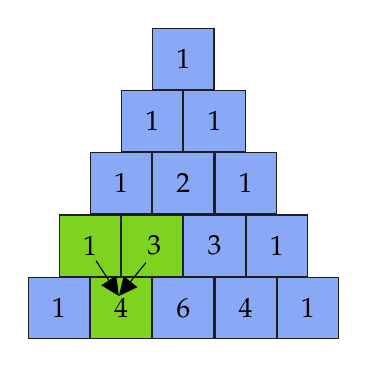
\begin{tikzpicture}[x=0.75pt,y=0.75pt,yscale=-1,xscale=1]
%uncomment if require: \path (0,300); %set diagram left start at 0, and has height of 300

%Shape: Square [id:dp6941490808398538] 
\draw  [color={rgb, 255:red, 31; green, 31; blue, 31 }  ,draw opacity=1 ][fill={rgb, 255:red, 137; green, 169; blue, 247 }  ,fill opacity=1 ] (192.5,0.33) -- (222,0.33) -- (222,29.83) -- (192.5,29.83) -- cycle ;

%Shape: Square [id:dp5483734211163716] 
\draw  [color={rgb, 255:red, 31; green, 31; blue, 31 }  ,draw opacity=1 ][fill={rgb, 255:red, 137; green, 169; blue, 247 }  ,fill opacity=1 ] (177.5,30.33) -- (207,30.33) -- (207,59.83) -- (177.5,59.83) -- cycle ;

%Shape: Square [id:dp6113568187175975] 
\draw  [color={rgb, 255:red, 31; green, 31; blue, 31 }  ,draw opacity=1 ][fill={rgb, 255:red, 137; green, 169; blue, 247 }  ,fill opacity=1 ] (207.5,30.33) -- (237,30.33) -- (237,59.83) -- (207.5,59.83) -- cycle ;

%Shape: Square [id:dp18321491615395535] 
\draw  [color={rgb, 255:red, 31; green, 31; blue, 31 }  ,draw opacity=1 ][fill={rgb, 255:red, 137; green, 169; blue, 247 }  ,fill opacity=1 ] (162.5,60.33) -- (192,60.33) -- (192,89.83) -- (162.5,89.83) -- cycle ;

%Shape: Square [id:dp5935951134760318] 
\draw  [color={rgb, 255:red, 31; green, 31; blue, 31 }  ,draw opacity=1 ][fill={rgb, 255:red, 137; green, 169; blue, 247 }  ,fill opacity=1 ] (192.5,60.33) -- (222,60.33) -- (222,89.83) -- (192.5,89.83) -- cycle ;
%Shape: Square [id:dp15135091580108684] 
\draw  [color={rgb, 255:red, 31; green, 31; blue, 31 }  ,draw opacity=1 ][fill={rgb, 255:red, 137; green, 169; blue, 247 }  ,fill opacity=1 ] (222.5,60.33) -- (252,60.33) -- (252,89.83) -- (222.5,89.83) -- cycle ;

%Shape: Square [id:dp6959691378679023] 
\draw  [color={rgb, 255:red, 31; green, 31; blue, 31 }  ,draw opacity=1 ][fill={rgb, 255:red, 126; green, 211; blue, 33 }  ,fill opacity=1 ] (147.5,90.33) -- (177,90.33) -- (177,119.83) -- (147.5,119.83) -- cycle ;

%Shape: Square [id:dp3401786459744438] 
\draw  [color={rgb, 255:red, 31; green, 31; blue, 31 }  ,draw opacity=1 ][fill={rgb, 255:red, 126; green, 211; blue, 33 }  ,fill opacity=1 ] (177.5,90.33) -- (207,90.33) -- (207,119.83) -- (177.5,119.83) -- cycle ;
%Shape: Square [id:dp054113641995666484] 
\draw  [color={rgb, 255:red, 31; green, 31; blue, 31 }  ,draw opacity=1 ][fill={rgb, 255:red, 137; green, 169; blue, 247 }  ,fill opacity=1 ] (207.5,90.33) -- (237,90.33) -- (237,119.83) -- (207.5,119.83) -- cycle ;
%Shape: Square [id:dp11590999892335718] 
\draw  [color={rgb, 255:red, 31; green, 31; blue, 31 }  ,draw opacity=1 ][fill={rgb, 255:red, 137; green, 169; blue, 247 }  ,fill opacity=1 ] (237.5,90.33) -- (267,90.33) -- (267,119.83) -- (237.5,119.83) -- cycle ;

%Shape: Square [id:dp23803207337642562] 
\draw  [color={rgb, 255:red, 31; green, 31; blue, 31 }  ,draw opacity=1 ][fill={rgb, 255:red, 137; green, 169; blue, 247 }  ,fill opacity=1 ] (132.5,120.33) -- (162,120.33) -- (162,149.83) -- (132.5,149.83) -- cycle ;

%Shape: Square [id:dp5531375567623269] 
\draw  [color={rgb, 255:red, 31; green, 31; blue, 31 }  ,draw opacity=1 ][fill={rgb, 255:red, 126; green, 211; blue, 33 }  ,fill opacity=1 ] (162.5,120.33) -- (192,120.33) -- (192,149.83) -- (162.5,149.83) -- cycle ;
%Shape: Square [id:dp4320593415188343] 
\draw  [color={rgb, 255:red, 31; green, 31; blue, 31 }  ,draw opacity=1 ][fill={rgb, 255:red, 137; green, 169; blue, 247 }  ,fill opacity=1 ] (192.5,120.33) -- (222,120.33) -- (222,149.83) -- (192.5,149.83) -- cycle ;
%Shape: Square [id:dp02227383517383874] 
\draw  [color={rgb, 255:red, 31; green, 31; blue, 31 }  ,draw opacity=1 ][fill={rgb, 255:red, 137; green, 169; blue, 247 }  ,fill opacity=1 ] (222.5,120.33) -- (252,120.33) -- (252,149.83) -- (222.5,149.83) -- cycle ;
%Shape: Square [id:dp7593605515111705] 
\draw  [color={rgb, 255:red, 31; green, 31; blue, 31 }  ,draw opacity=1 ][fill={rgb, 255:red, 137; green, 169; blue, 247 }  ,fill opacity=1 ] (252.5,120.33) -- (282,120.33) -- (282,149.83) -- (252.5,149.83) -- cycle ;

%Straight Lines [id:da6208300176170172] 
\draw [color={rgb, 255:red, 0; green, 0; blue, 0 }  ,draw opacity=1 ]   (165.17,112.33) -- (175.08,127.65) ;
\draw [shift={(176.17,129.33)}, rotate = 237.09] [fill={rgb, 255:red, 0; green, 0; blue, 0 }  ,fill opacity=1 ][line width=0.75]  [draw opacity=0] (8.93,-4.29) -- (0,0) -- (8.93,4.29) -- cycle    ;

%Straight Lines [id:da8782482964882432] 
\draw [color={rgb, 255:red, 0; green, 0; blue, 0 }  ,draw opacity=1 ]   (189.17,113.33) -- (177.43,127.78) ;
\draw [shift={(176.17,129.33)}, rotate = 309.09000000000003] [fill={rgb, 255:red, 0; green, 0; blue, 0 }  ,fill opacity=1 ][line width=0.75]  [draw opacity=0] (8.93,-4.29) -- (0,0) -- (8.93,4.29) -- cycle    ;


% Text Node
\draw (207.25,15.08) node  [align=left] {1};
% Text Node
\draw (192.25,45.08) node  [align=left] {1};
% Text Node
\draw (222.25,45.08) node  [align=left] {1};
% Text Node
\draw (207.25,75.08) node  [align=left] {2};
% Text Node
\draw (177.25,75.08) node  [align=left] {1};
% Text Node
\draw (237.25,75.08) node  [align=left] {1};
% Text Node
\draw (193.25,105.08) node  [align=left] {3};
% Text Node
\draw (162.25,105.08) node  [align=left] {1};
% Text Node
\draw (252.25,105.08) node  [align=left] {1};
% Text Node
\draw (222.25,105.08) node  [align=left] {3};
% Text Node
\draw (177.25,135.08) node  [align=left] {4};
% Text Node
\draw (207.25,135.08) node  [align=left] {6};
% Text Node
\draw (147.25,135.08) node  [align=left] {1};
% Text Node
\draw (267.25,135.08) node  [align=left] {1};
% Text Node
\draw (237.25,135.08) node  [align=left] {4};

\end{tikzpicture}
\end{minipage}
\begin{minipage}{0.6\linewidth}

\begin{itemize}
	\item	Triangle des coefficients binomiaux
	\item 	Chaque nombre est la somme des 2 nombres directement au-dessus.
\end{itemize}

\begin{align*}
	\binom{n}{k}
		&=	\binom{n - 1}{k - 1} + \binom{n - 1}{k}		\\
\end{align*}
\end{minipage}

\subsection*{Moments}

\begin{tabular}{| l | l |}
\hline
	Moment d'ordre $n$ \textit{(autour de l'origine)}.	&	$\text{E}[X^{n}] = \underset{i}{\sum} x_{i}^{n} \Pr(X = x_{i})$	\\
	Moment \textbf{\textit{centré}} d'ordre $n$.	&	$\text{E}[(X - \text{E}[X])^{n}] = \underset{i}{\sum} (x_{i} - \text{E}[X])^{n} \Pr(X = x_{i})$	\\
	Moment \textbf{\textit{réduit}} d'ordre $n$.&	$\text{E}\left[\left(\frac{X}{\sqrt{\text{V}(X)}}\right)^{n}\right] = \underset{i}{\sum} \left(\frac{x_{i}}{\sqrt{\text{V}(X)}}\right)^{n} \Pr(X = x_{i})$	\\
	Moment \textbf{\textit{centré-réduit}} d'ordre $n$.	&	$\text{E}\left[\left(\frac{X - \text{E}[X]}{\sqrt{\text{V}(X)}}\right)^{n}\right] = \underset{i}{\sum} \left(\frac{x_{i} - \text{E}[X]}{\sqrt{\text{V}(X)}}\right)^{n} \Pr(X = x_{i})$	\\
	Coefficient d'asymétrie \textit{(\textbf{Skewness})} 	&	$\gamma_{X} = \text{E}\left[\left(\frac{X - \text{E}[X]}{\sqrt{\text{V}(X)}}\right)^{3}\right]$	\\
	Coefficient d'aplatissement \textit{\textbf{(Kurtosis)}} 	&	$\kappa_{X} = \text{E}\left[\left(\frac{X - \text{E}[X]}{\sqrt{\text{V}(X)}}\right)^{4}\right]$	\\
	Fonction stop-loss 	&	$\pi_{X}(d) = \text{E}\left[\max(X - d; 0)\right]$	\\
	Fonction d'excès-moyen 	&	$\pi_{X}(d) = \text{E}\left[X - d | X > d\right]$	\\	\hline
\end{tabular}

\textbf{Conditionnels}
\begin{align*}
	\text{E}[X]	&=	\text{E}_{Y}[\text{E}[X|Y]]	&
	\text{V}(X)	&=	\text{E}_{Y}[\text{V}(X|Y)] + \text{V}_{Y}(\text{E}[X|Y])
\end{align*}

\begin{align*}
	\text{Cov}(X, Y)	
		&=	\text{E}[XY] - \text{E}[X] \text{E}[Y]	
\end{align*}

\begin{enumerate}
	\item $\text{Cov}(X, Y) = \text{Cov}(Y, X)$
	\item $\text{Cov}(X, X) = \text{V}(X)$
	\item $\text{Cov}(X, Y) \overset{\bot}{=} 0$
	\item $\text{Cov}(c, X) = 0$
	\item $\text{Cov}(cX, Y) = c\text{Cov}(X, Y)$
	\item $\text{Cov}(\sum_{i = 1}^{n}\alpha_{i} X_{i}, \sum_{j = 1}^{m}\beta_{j} Y_{j}) = \sum_{i = 1}^{n}\sum_{j = 1}^{m}\alpha_{i}\beta_{j}  \text{Cov}(X_{i}, Y_{j})$
\end{enumerate}

\begin{align*}
	\text{V}(\sum_{i = 1}^{n}\alpha_{i} X_{i}) 
		&= \sum_{i = 1}^{n}\sum_{j = 1}^{m}\alpha_{i}^{2}\text{V}(X_{i}) + 2 \underset{i < j}{\sum\sum} \alpha_{i}\alpha_{j} \text{Cov}(X_{i}, X_{j})	\\
	\rho_{\textrm{P}}(X, Y)
		&=	\frac{\text{Cov}(X, Y)}{\sigma_{X}\sigma_{Y}}
\end{align*}

\subsubsection*{Convolution}
\begin{align*}
	f_{X + Y}(s)	
		&=	\int_{-\infty}^{\infty} f_{X}(s - y) f_{Y}(y) dy	
\end{align*}

\subsection*{Lois multivariées}
	
\textbf{Loi multinomiale}
\begin{align*}
	\Pr(X_{1} = x_{1}, \dots, X_{r} = x_{r})
		&=	\binom{n}{x_{1}, \dots, x_{r}} p_{1}^{x_{1}} \dots p_{r}^{x_{r}}
\end{align*}

\textbf{Loi normale multivariée}
\begin{align*}
	f_{\matr{X}}(\matr{x}) 
		&= 	\frac{1}{(2 \pi)^{\frac{n}{2}} \sqrt{\text{det}(\bm{\Sigma})}} \e{\shortminus \frac{1}{2} (\matr{x} - \bm{\mu})^{\top} \bm{\Sigma}^{-1}(\bm{x} - \bm{\mu})}
\end{align*}

\end{multicols*}


\end{document}
